\begin{frame}
    \frametitle{ICube, un laboratoire pluridisciplinaire}
    \framesubtitle{Une force de recherche majeure à Strasbourg (760 personnes)}
    ICube existe depuis le 1$^{er}$ Janvier 2013 :
        \begin{itemize}
            \item un laboratoire de recherche en \textbf{ingénierie}, en \textbf{informatique} et en \textbf{imagerie} avec comme secteurs d'activités privilégiés la \textbf{santé}, l'\textbf{environnement} et le \textbf{développement durable}.
        \end{itemize}
        \begin{center}
            \begin{tikzpicture}[]
                \node (image) at (current page.center) {
\includegraphics[scale=0.25]{logos/icube/icube-short.png}};
                \node[align=center,yshift=-0.75cm] at (current page.center) {Imagerie};        
                \node[align=center,xshift=-1.5cm] at (current page.center) {Ingénierie};   
                \node[align=center,xshift=1.5cm] at (current page.center) {Informatique};                               
            \end{tikzpicture}
        \end{center}
        \begin{itemize}
            \item une unité mixte de recherche (UMR7357) sous la cotutelle de l’\textbf{université de Strasbourg}, du \textbf{CNRS}, de l’\textbf{INSA Strasbourg}, de l’\textbf{ENGEES} et de l’\textbf{INRIA Grand Est}.
        \end{itemize}
    \begin{figure}[!h]
        \centering
            
\includegraphics[height=0.8cm]{inria/inr_logo_rouge.png}
            
\includegraphics[height=0.8cm]{engees/ENGEES_CMJN_png.png}
            
\includegraphics[height=0.8cm]{insa_strasbourg/Logo_INSAvilleStrasbourgCourt-pantone_marge.jpg}
            
\includegraphics[height=0.8cm]{cnrs/LOGO_CNRS_BLEU.png}
            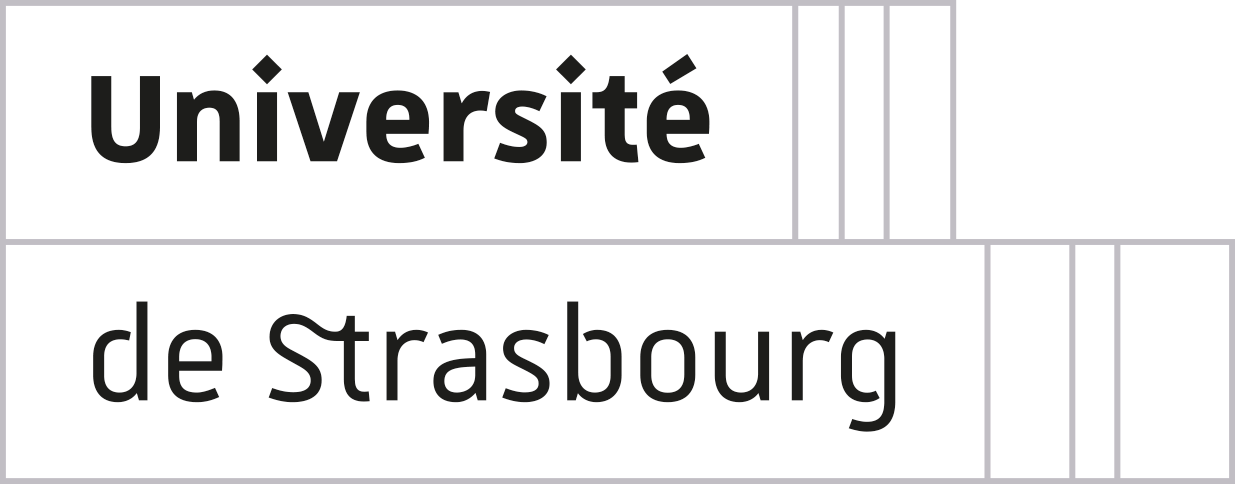
\includegraphics[height=0.8cm]{unistra/signature-universite-minimale-couleur_03.png}
    \end{figure}
    \begin{itemize}
        \item avec comme partenaires privilégiés :
    \end{itemize}
    \begin{figure}[!h]
        \centering
            
\includegraphics[height=0.8cm]{partenaires.png}
    \end{figure}    
\end{frame}